\chapter{}\label{ex:aufg4}
%
\section{}\label{sec:aufg4a}
Im Bereich eines kompletten Phasendurchlaufes, wie die blaue obere Kurve in in Abb. \ref{fig:aufgenommen_hallSensorSig} zeigt, finden zwei Perioden des Hallsensorsignals statt, dadurch ergibt sich eine Polpaarzahl von zwei. Dies wird durch die Formel \ref{for:poolpaarZahl} best\"atigt.
\begin{figure}[htb]
	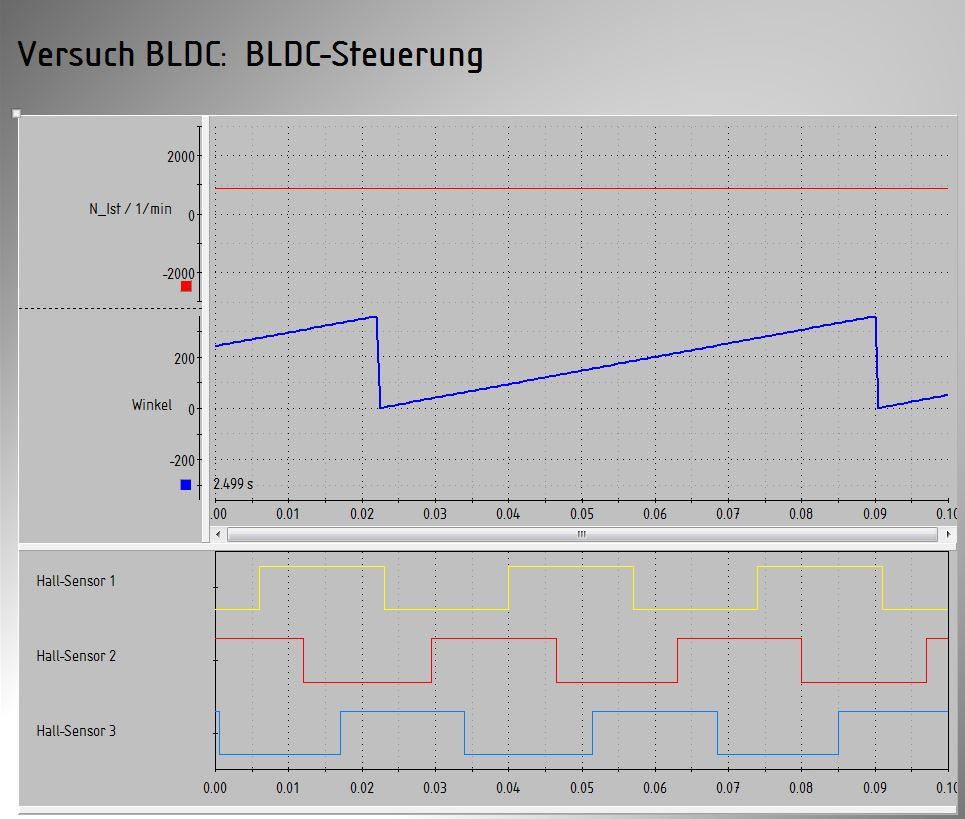
\includegraphics[width = \textwidth]{./Bilder/bldc_aufgenommenSig}
	\caption{Aufgenommene Hallsensorsignale}
	\label{fig:aufgenommen_hallSensorSig}
\end{figure}
\newpage
\section{}\label{sec:aufg4b}
Im der folgenden Tabelle (siehe Tab. \ref{tab:T_Ansteuerung}) wird der Ansteuerwert für jeden Transistor dargestellt, der für jedes Hallsensorsignal in Frage kommt um eine Drehung zu verursachen.

\begin{table}[htb]
	\centering
\begin{tabular}{ccc||cccccc}
	$H_1$ & $H_2$ & $H_3$ & $U_{HS}$ & $U_{LS}$ & $V_{HS}$ & $V_{LS}$ & $W_{HS}$ & $W_{LS}$ \\ 
	0&0&0&0&0&0&0&0&0\\
	0&0&1&0&0&1&0&0&1\\
	0&1&0&1&0&0&1&0&0\\
	0&1&1&1&0&0&0&0&1\\
	1&0&0&0&1&0&0&1&0\\
	1&0&1&0&1&1&0&0&0\\
	1&1&0&0&0&0&1&1&0\\
	1&1&1&0&0&0&0&0&0
\end{tabular}  
\caption{Wertetabelle zur Ansteuerung der Transistoren}
\label{tab:T_Ansteuerung}
\end{table}
%
\section{}\label{sec:aufg4c}
%
Die Implementierung erfolgte in Matlab/Simulink.